\section{Schematics}
\label{app:schematics}
\subsection{Analog board}

% \newpage
% \begin{hugepage}
% \subsection{AMS Slave PCB}\label{sec:app:amsslave}

% \pdfpagewidth=2\pdfpagewidth
% \begin{figure}
%   \centering
%   \includepdf[pages=1,scale=1.45,offset=200 -30,pagecommand={\pagestyle{fancy}}]{07-Appendix/AMS_Slave_PCB.pdf}

% \end{figure}
% \end{hugepage}
% \newpage






\begin{figure} [H]
  \centering
  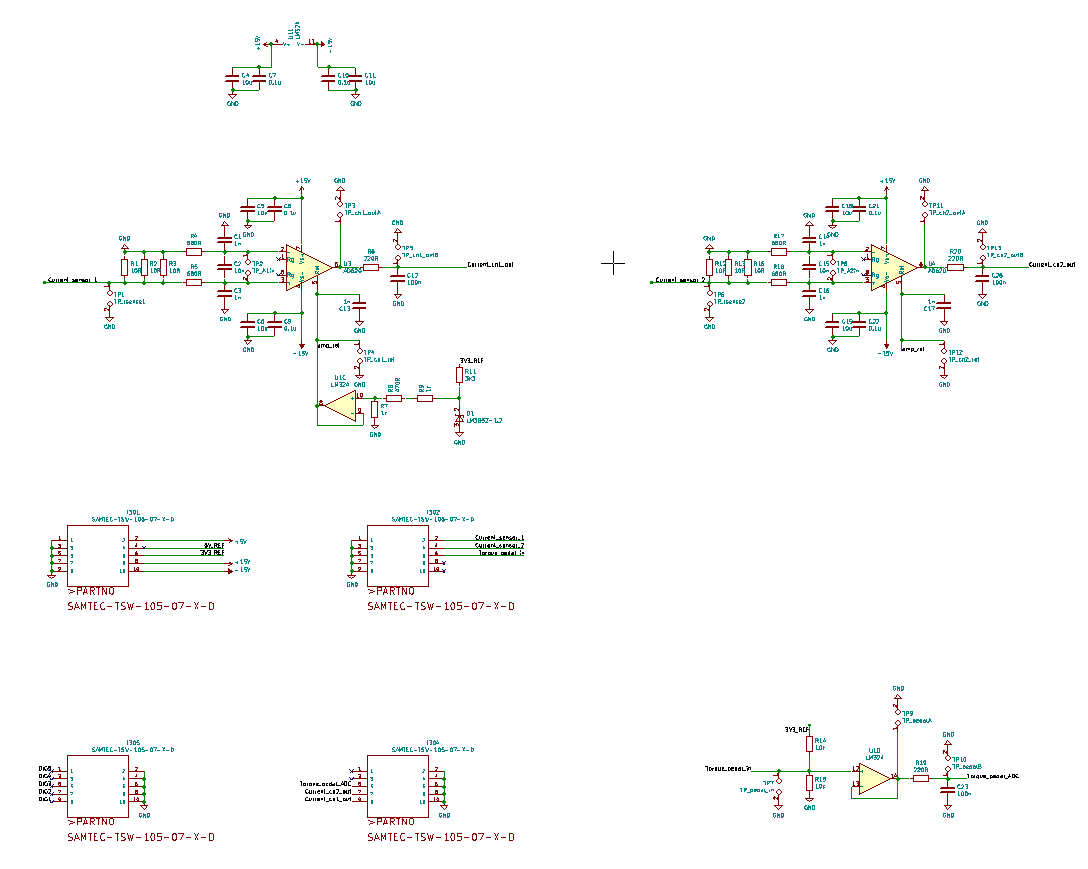
\includegraphics[width=\linewidth]{pictures/hardware/Analog_Interface_board/analog_schematic.png}
  \caption{The analog board circuit schematic}
  \label{fig:analog_schematic}
\end{figure}

\begin{figure} [H]
  \centering
  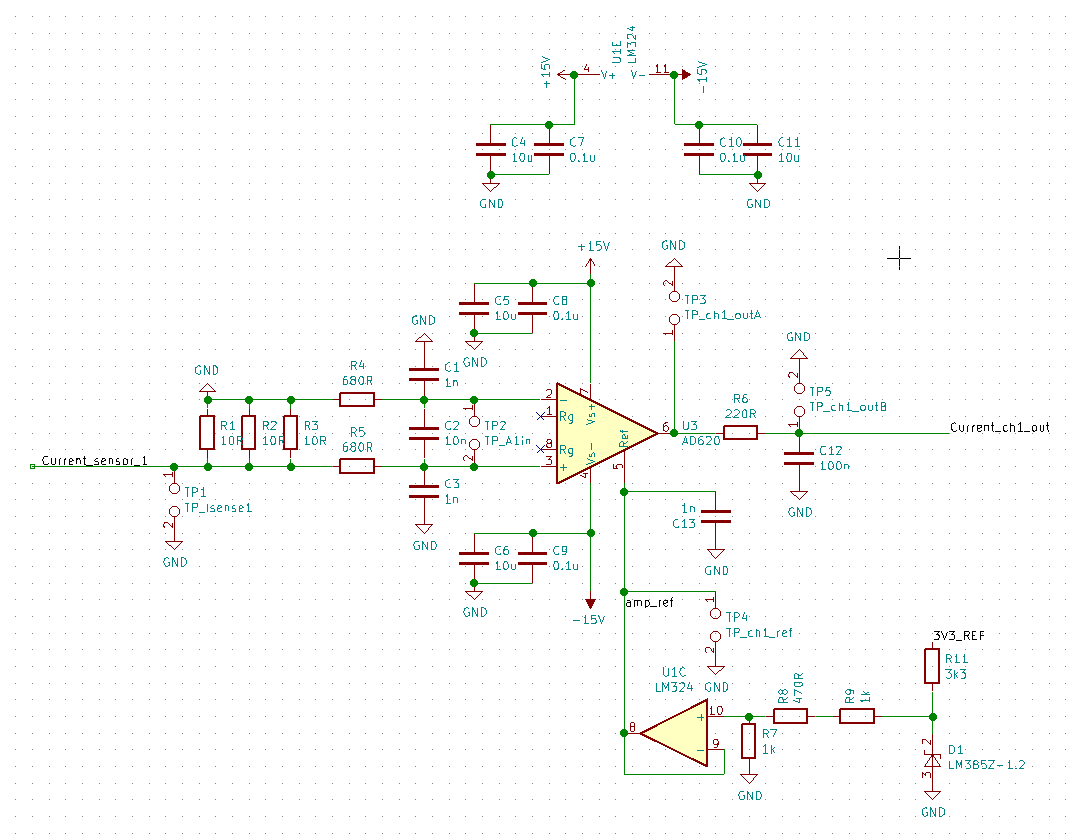
\includegraphics[width=\linewidth]{pictures/hardware/Analog_Interface_board/analog_ch1.png}
  \caption{The analog board current transducer channel 1 and the amplifier supply decoupler capacitors}
  \label{fig:analog_ch1}
\end{figure}

\begin{figure} [H]
  \centering
  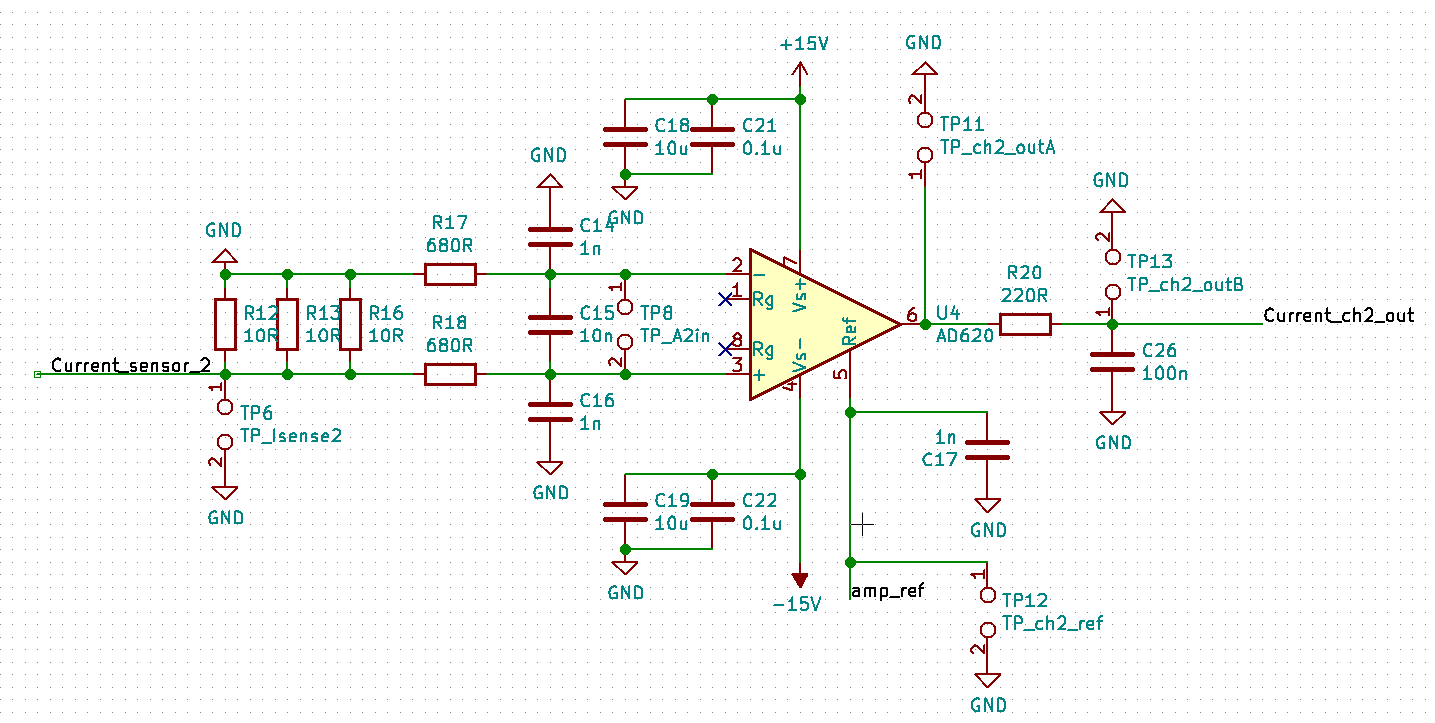
\includegraphics[width=\linewidth]{pictures/hardware/Analog_Interface_board/analog_ch2.png}
  \caption{The analog board current transducer channel 2}
  \label{fig:analog_ch2}
\end{figure}

\begin{figure} [H]
  \centering
  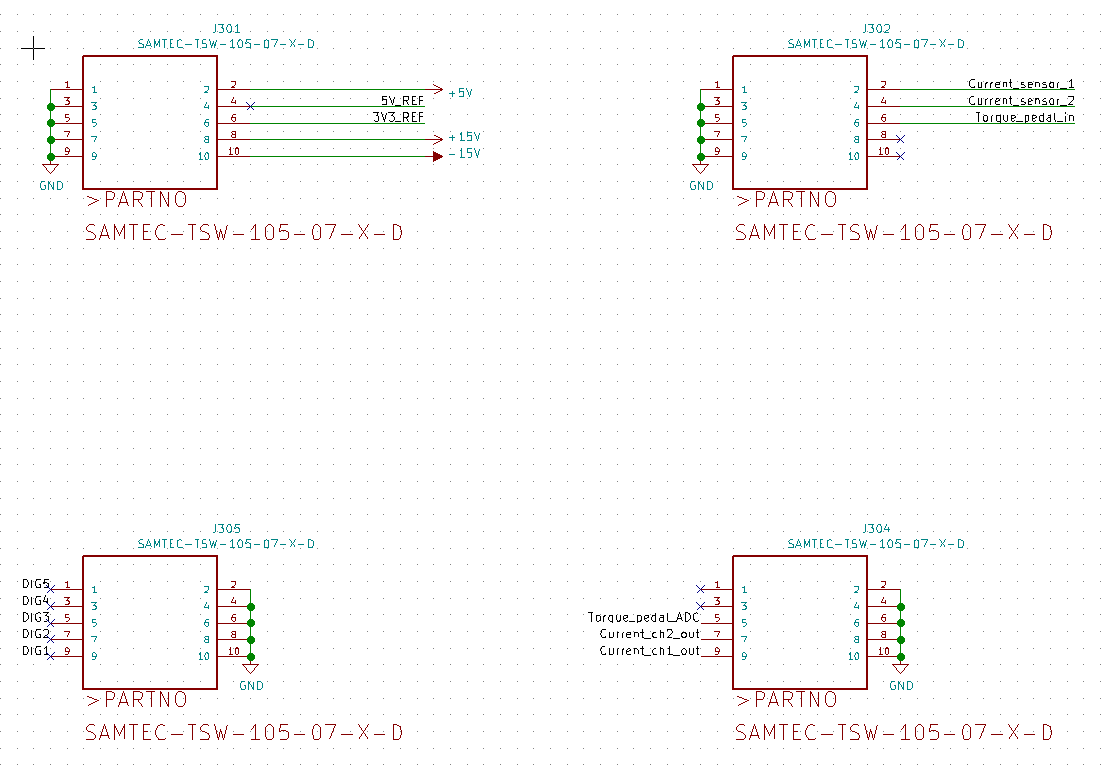
\includegraphics[width=\linewidth]{pictures/hardware/Analog_Interface_board/analog_connectors.png}
  \caption{The analog board connectors to the main board}
  \label{fig:analog_connector}
\end{figure}

\begin{figure} [H]
  \centering
  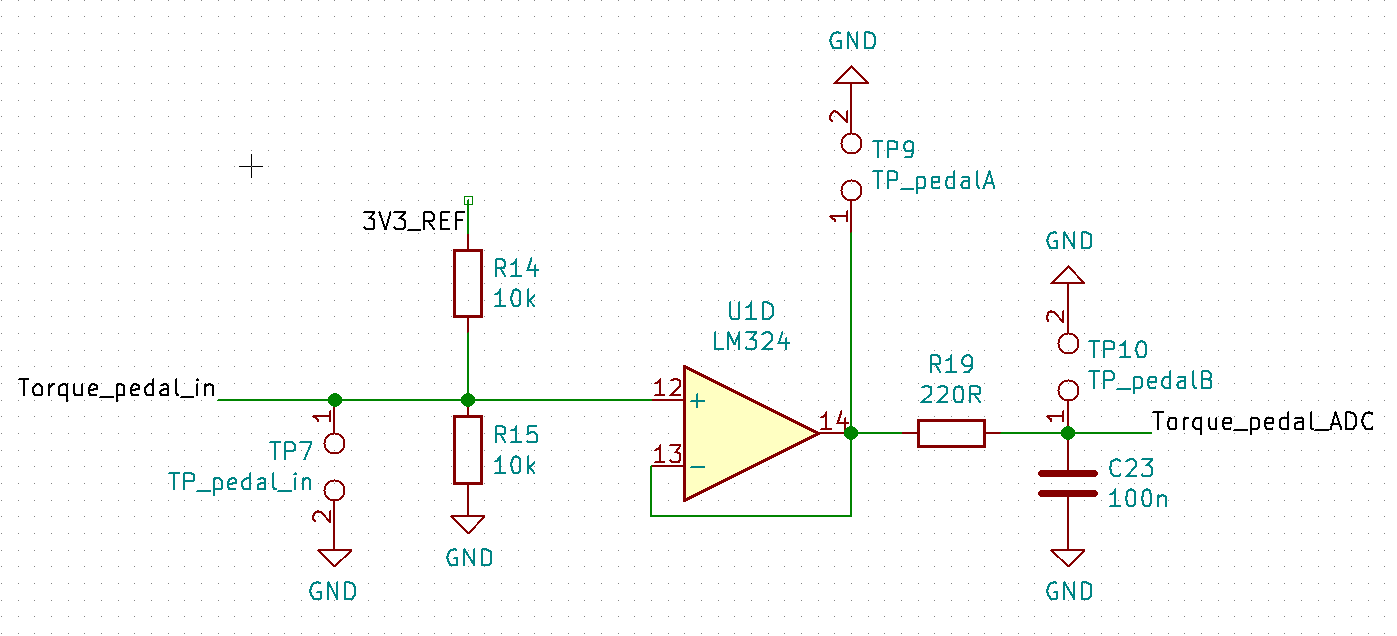
\includegraphics[width=\linewidth]{pictures/hardware/Analog_Interface_board/torque_pedal_divider.png}
  \caption{The analog board circuit schematic}
  \label{fig:analog_torque_pedal}
\end{figure}

\subsection{Driver board}

\begin{figure} [H]
  \centering
  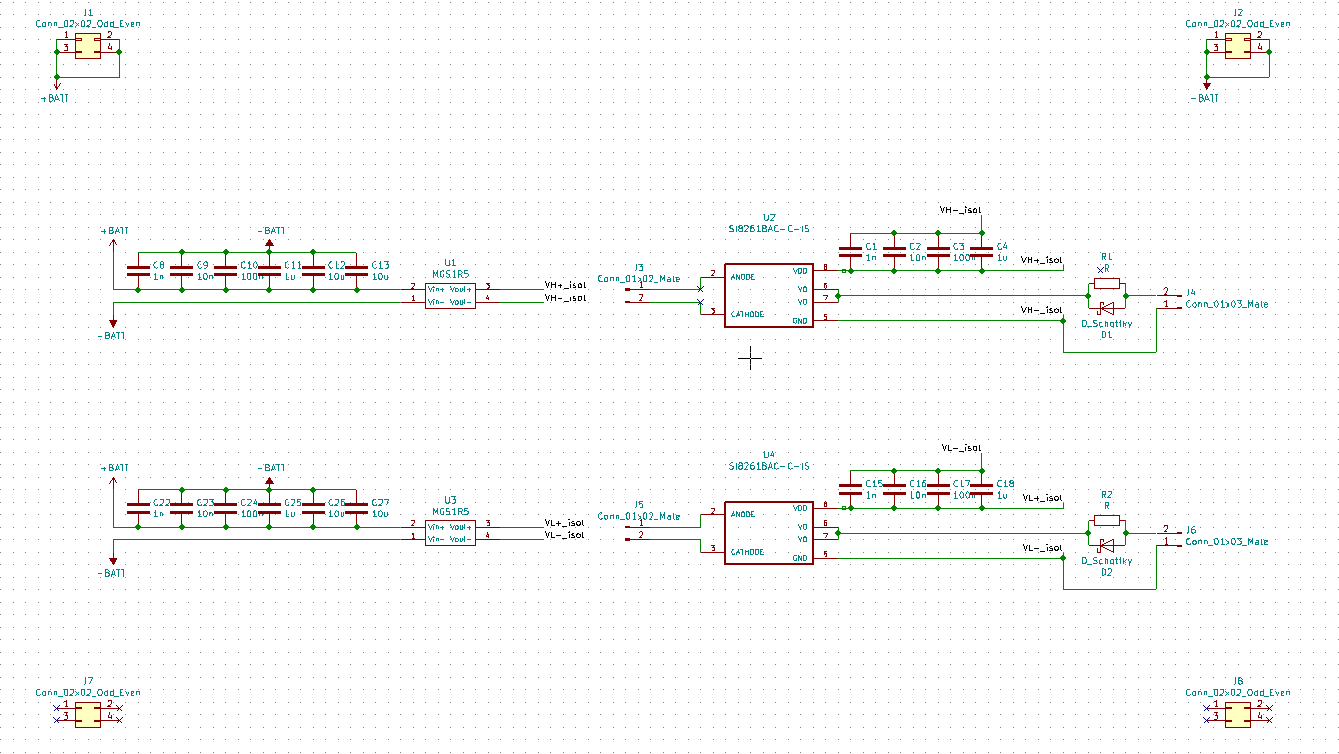
\includegraphics[width=\linewidth, angle = 90]{pictures/hardware/Driver_Board/driver_schematic.png}
  \caption{The driver board circuit schematic}
  \label{fig:driver_schematic}
\end{figure}

\subsection{Power board}